\documentclass{article}
\usepackage{tikz}
\usepackage{xcolor}
\begin{document}
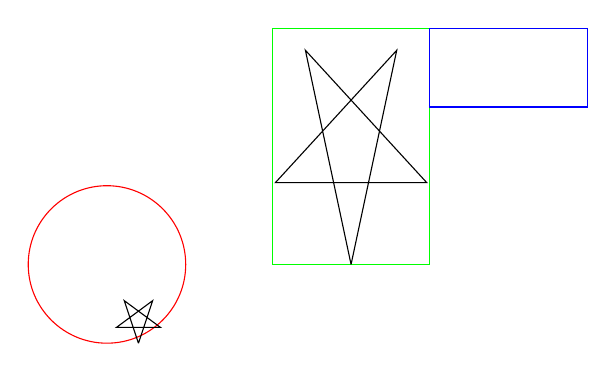
\begin{tikzpicture}
\definecolor{myColor}{RGB}{255,0,0}
\draw[myColor] (0.9,2) circle (1cm);
\definecolor{myColor}{RGB}{0,255,0}
\draw[myColor] (3,2) rectangle (5,5);
\definecolor{myColor}{RGB}{0,0,255}
\draw[myColor] (5,4) rectangle (7,5);
\definecolor{myColor}{RGB}{0,0,0}
\draw[myColor] (1.3,1) -- (1.48,1.54) -- (1.02,1.2) -- (1.58,1.2) -- (1.12,1.54) -- (1.3,1);
\definecolor{myColor}{RGB}{0,0,0}
\draw[myColor] (4,2) -- (4.58,4.72) -- (3.04,3.04) -- (4.96,3.04) -- (3.42,4.72) -- (4,2);
\end{tikzpicture}
\end{document}
